\documentclass[12pt,a4paper]{article}
\usepackage[utf8]{inputenc}
\usepackage[english]{babel}
\usepackage{amsmath}
\usepackage{amsfonts}
\usepackage{amssymb}
\usepackage{graphicx} 
\usepackage[left=2cm,right=2cm,top=2cm,bottom=2cm]{geometry}
\usepackage{hyperref}
\author{Adrian Bach}
\title{Using artificial intelligence to improve decision-making in conservation conflicts \\\medskip Ten-week report}

% bibliography 
\usepackage{natbib}
\bibliographystyle{humannat}

\begin{document}
\maketitle

%\newpage
\tableofcontents

\newpage
\section{Context}
\subsection{Conservation}

% 6th mass extinction? Ref: ----------------------------------------------------
% Ceballos, G., Ehrlich, P. R., & Dirzo, R. (2017). Biological annihilation via the ongoing sixth mass extinction signaled by vertebrate population losses and declines. Proceedings of the National Academy of Sciences, 114(30), E6089--E609. https://doi.org/10.1073/pnas.1704949114
% R\'{e}gnier, C., Achaz, G., Lambert, A., Cowie, R. H., Bouchet, P., & Fontaine, B. (2015). Mass extinction in poorly known taxa. Proceedings of the National Academy of Sciences, 112(25), 201502350. https://doi.org/10.1073/pnas.1502350112
% Dirzo, R., Young, H. S., Galetti, M., Ceballos, G., Isaac, N. J. B., & Collen, B. (2014). Defaunation in the Anthropocene. Science, 345(6195), 401–406. https://doi.org/10.1126/science.1251817
% Importance of ecosystem services: --------------------------------------------
% Tilman, D., Isbell, F., & Cowles, J. M. (2014). Biodiversity and Ecosystem Functioning. Annual Review of Ecology, Evolution, and Systematics, 45, 471–493. https://doi.org/10.1126/science.1064088
% Hautier, Y., Tilman, D., Isbell, F., Seabloom, E. W., Borer, E. T., & Reich, P. B. (2015). Anthropogenic environmental changes affect ecosystem stability via biodiversity. Science, 348(6232), 336–340.
% Venail, P., Gross, K., Oakley, T. H., Narwani, A., Allan, E., Flombaum, P., ... Cardinale, B. J. (2015). Species richness, but not phylogenetic diversity, influences community biomass production and temporal stability in a re-examination of 16 grassland biodiversity studies. Functional Ecology, n/a-n/a. https://doi.org/10.1111/1365-2435.12432
Human survival depends on the services ecosystems provide, such as pollination, soil enrichment, water treatment, and carbon dioxide fixation, among many more.
% BRAD It seems like you have two separate points here supporting your first sentence (that preserving biodiversity is a central concern for humanity). I suggest breaking them down into two separate sentence for clarity. See above reference suggestions (and references therein) for the importance of biodiversity for fulfilling  key ecosystem functions. 
Additionally, nature play an increasingly recognized role in human mental well-being, and is often an inspiration for technological, cultural, and artistic innovations.
% BRAD Examples or reference? Could also mention cultural or artistic innovation?
% BRAD `important' or perhaps `fundamental'? This part was slightly unclear to me at first. I assume that this is slightly different from your point about human survival? I.e., something like human happiness and culture associated with nature? I'm not sure what the best references would be for this, though I agree it would be good to include one or two. Nils or John Wilson might be good sources for finding this in the social literature. Also, see these potential links --> https://www.pnas.org/content/early/2015/06/23/1510459112 and https://www.ncbi.nlm.nih.gov/pmc/articles/PMC5744722/
A key for ensuring ecosystem sustainability is the maintenance of biodiversity, which enables quick and dynamic responses to change.
% Need to specify what about diveresity (i.e., diversity is key -- but what does this mean; having a lot of it, not a lot?). Also, `permanence' seemed a bit strong. I would be slightly cautious about suggesting that the long-term maintenance of ecosystems is ensured by diversity. At worst, this could be tautological or ambiguous (because you've not explained by what you mean by ecosystem permanence/sustainability -- does this just mean that some fraction of biodiversity persists, that key ecosystem functions persist, or something else?). I believe that Iagree with the general idea though -- which I interpret as a biodiverse ecosystem is likely to be more able to adapt to changing conditions. I'll try to think of a good reference for this, but you'll want to be careful to avoid equating biodiversity with ecosystem stability (or, at least, reference very carefully, as there is considerable debate over whether or not more complex -- i.e., diverse -- ecological systems are more or less 'stable' -- depends on how stability is defined).
Thus, at the beginning of this new mass extinction episode, conservation of biodiversity is a vital concern for humanity.
% BRAD See commented references above. Also, I don't think it's necessary to be ambiguous about a new mass extinction event -- the evidence is probably strong enough now to state that we're in a sixth mass extinction unequivicolly.conservation of biodiversity is currently at the center of the . % I'm not sure if I would describe conservation as a field in ecology. Perhaps you could make an even stronger statement here though -- e.g., `Hence, conservation of biodiversity is critical for human survival and well-being, and remains a defining global challenge for the twenty-first century', or something like it?
%One of the many aspects, intense competition/antagonism between human activity and wildlife. Ref: \\
%Conservation as a way to tame this problem. Ref: \\
%
%\subsection{Conservation}

%According to ... Definition of conservation. (to complete tomorrow morning)\\
% BRAD I don't think that you need to define conservation explicitly (especially because you talk about conservation in the preceding paragraph, so it doesn't make much sense to define here). I do like the focus on different ways of doing conservation biology, so an opening sentence introducing the idea that there are many ways to do conservation would be good.
%Different kinds of conservation actions.
Conservation of biodiversity has taken many different forms.
% BRAD Here's where I think some definitions might be useful; you introduce these different ways conservation can be applied, with really useful examples, but it might make sense to define different ways of doing conservation (giving each its own sentence), then listing some examples (from the reader's perspective, I assume the distinctions will become important later). I think that the examples you provide are good ones, but it might be useful to go into just a bit more detail about them -- e.g., how are `monetary incentives' useful for applying conservation (i.e., how would you explain the idea to a biologist who was not very familiar with conservation?). 
For example, protected areas has been established to preserve intact ecosystems from human impact, like in Scotland where the goose population were granted Special Protection Areas to feed \cite{bainbridge2017goose}, or in the Kruger National Park in Africa where approximately two million hectares of wooded savanna has been secured for management of its biodiversity \cite{vanwilgen2011critical}.
The same method has been applied to already damaged ecosystems in order to restore them.
For instance, in \citep{rumpff2011state}, conservation managers prevented access to several previously logged areas in order to promote vegetation regrowth, influencing which kind of habitat would emerge from them. 
%: protection areas, ?. Ref: Wilgen2011, Brainbridge2017.
Conservation strategies have also been developed in reaction to ongoing problems without preventing contact.
In Scotland, to protect geese from being culled when grazing on farmers' crop, Scotland provided monetary compensations for the yield loss in exchange for the farmers to allow undisturbed grazing \citep{bainbridge2017goose, cusack2018time}.
% BRAD I'm wondering if the wording should be slightly different here -- rather than conservation `being applied', would it make more sense to talk about management applications for the purpose of conservation goals?
Another example is offsetting, which is balancing "local habitat destruction by restoring, enhancing and/or protecting similar but separate habitat" \citep{gordon2011assessing}.
In this case study, some of the native habitat destroyed by Melbourne's growing urbanisation was compensated by the introduction of the same habitat further away the State.
% BRAD Can you give an example of an offsetting case study here? 
%But conserving a species for its own sakes sometimes lead it to reach numbers being problematic for human activities. Ref: Redpath's book.
But these implementations, just as any in conservation, faced many different challenges \citep{keith2011uncertainty, vanwilgen2011critical}.\\
% BRAD I think more is needed here -- including perhaps one example of successful implementation? Also, I'm not sure what you mean by `many other examples' -- do you mean examples of case studies, or examples of ways in which conservation can be applied? I think some sort of summary is missing here; if the point is that conservation success is rare (is it?), can you maybe talk a bit about the advantages and disadvantages of these different applications, or perhaps what is missing from these different approaches? How does this paragraph relate to the previous one? 
% This last sentences might actually fit better as the first sentence of a next pararaph, or maybe better, can you list the numerous challenges faced explicitly here; this would introduce the challenges to the reader and help them link the points of the first two paragraphs with the specific topics that follow. 
%
%\subsection{Problems faced}

%\subsubsection{Complexity}
Indeed, the systems conservation deals with are highly complex and densely interconnected, linking ecology to sociology, agronomy and climatology simultaneously. % I'm not entirely sure what is meant by 'densely' interconnected. 
They exhibit the characteristics of wicked problems, including "\textit{numerous interacting elements lacking any central control, non-linear interactions between elements, constant change which is seldom reversible, and no clearly defined boundaries}" \citep{game2013conservation}.
% BRAD I think you can probably say 'all' instead of 'most'. Or, if not, what characteristics of complex systems are socio-ecological systems lacking? Potentially useful references here:
% Sharman, M., & Mlambo, M. C. (2012). Wicked: The problem of biodiversity loss. Gaia, 21(4), 274–277.
% Brodie, J. F., Aslan, C. E., Rogers, H. S., Redford, K. H., Maron, J. L., Bronstein, J. L., & Groves, C. R. (2014). Secondary extinctions of biodiversity. Trends in Ecology & Evolution, 1–9. https://doi.org/10.1016/j.tree.2014.09.012
% Ascough, J. C., Maier, H. R., Ravalico, J. K., & Strudley, M. W. (2008). Future research challenges for incorporation of uncertainty in environmental and ecological decision-making. Ecological Modelling, 219(3–4), 383–399. https://doi.org/10.1016/j.ecolmodel.2008.07.015
%It makes their complete understanding out of our cognition.
%Ref: grimm1999individual, wilgen2011critical, runge2011uncertainty, schluter2013new,pretty much every article I've read.
In such systems, it is often impossible to isolate the causes of changes, and the response to a conservation policy is lost in other signals from a myriad of uncontrollable external factors.
For a small-scale simple example, the increase in goose population in the 80's in Scotland is not merely linked to the implementation of protection policy, but also to climate and land-use change \citep{mason2017changing}. And the larger the system is, the more numerous are the possible external causes for change.
% BRAD I think I see what you mean, but can you clarify what kinds of changes and causes you are talking about, maybe with an example (do you mean, e.g., knowing how much an ecosystem service such as pollination has been decreased by a rise in global temperature -- probably not the best example, but something like that?). I think the point you're making is an important one, but readers might have a difficult time following wihtout something concrete on which to focus.
Thus, monitoring a system's response to a policy over time can be very expensive, time consuming, and possibly intractable if the number of possible variables affecting conservation is large.
% BRAD I'm trying to think of some good references for this.  Also, I think it might be good to mention the above in the context of policy earlier. I infer from the line of reasoning here that it is very difficult to predict or understand the consequences of implementing some management action according to policy because socio-ecological systems are complex (creating difficulties for all of the reasons you state above). But it's not until this sentence that you introduce response to policy per se. Even a sentence prior to this one, just stating that all of the aforementioned factors make knowing the consequences of any sort of management intervention very difficult -- thus ``monitoring a system's...''. 
This results in conservation policies often lacking data to account for their effectiveness, or to understand failure \citep{keith2011uncertainty}.
% Furthermore, management is based on estimations of populations, which accuracy varies according to the technique \citep{BUNNEFELD2011441}.
% BRAD I think more is needed here, as it's the first time you mention populations (rather than, e.g., 'areas' or 'habitat'). Some sort of transition from the complex system to how a managed population will respond to change would be very helpful here; then it will be easier to understand why specific techniques associated with management can be problematic. Alternatively, it might be useful to introduce a new paragraph after "Consequently, conservation..." to introduce the idea of management of populations, transitioning from the focus on large complex socio-ecological systems to looking at just one managed population (with the broader context now established). You would then have the reader in the right frame of might to understand why managing even a single population can be very challenging, and you could more naturally focus on specific details of population management (e.g., estimates, uncertainty, etc.).
%Ref: rumff2011, all of the articles from the 2011 special edition.
To summarize, conservation faces uncertainty at many levels, in the sense that anticipating if the consequences of the policy will fulfil the conservation goals is very challenging.
% BRAD I think more is needed to explain this, as you've not used 'uncertainty' explicitly yet.

%\subsubsection{Rigidity}
This inability to predict the system's response to a change in the conservation policy can result in managers' reluctance to change, and in the maintain of inadequate conservation policies \citep{peterson2005conservation, keith2011uncertainty}.
% BRAD This paragraph goes back to talking about the whole system; this might make a good ending sentence before turning to population management. Also, 'reluctance to change' for whom? Managers, stakeholders, both?
%Ref: geese case, apply a simple protection lead to population reaching conflictual numbers.
%Other limits in keith2011uncertainty about politics and self-serving.
Moreover, conservation implementations often takes place in a political context, and can be significantly slowed, even blocked, by divergent political interests or lobbies for groups that would not benefit from the policy \citep{keith2011uncertainty}.
% BRAD Can clarify 'it' (e.g., 'population management')
%Unexpectedly but fortunately, there is little evidence that bigger budgets make conservation easier or more effective \citep{game2013conservation}.
% BRAD I'm not sure if this is the right place for this sentence -- it's interesting and important, but seems a bit out of place here. 

%Conservation had to be carried on despite these potentially discouraging barriers, acting on protection while dealing with them.
All the above led to the question: how to conduct efficient conservation, while dealing with these discouraging barriers and embracing uncertainty?

\subsection{Adaptive management}
%
%\subsection{Purpose}

%how it deals with certain problems. Acting while acquiring informations, learning from mistakes, closer to the system response to act as quickly as possible.
Adaptive Management (AM) is a decision-making process that dynamically updates management policy in response to the system's behaviour.
%This way, the conservation policy can be better fitted to the system, and 
Acting regularly allows managers to acquire information on how the system responds to change to update the policy heuristically.
% BRAD: Clarify `conservation' (e.g., `conservation methods' or `conservation procedures'?)
% BRAD: I'm not entirely sure I see how this sentence differs from or builds on the previous sentence.
%Uncertainty is an irreducible aspect of conservation, so it seems more relevant to act embracing it rather than waiting and keep on with an inadequate policy.
Although AM also relies on the monitoring of a set of variables, the choice of these variables can be adapted according to the problems detected along policy updates. 
% BRAD: I'm not sure I follow this well -- can you give an example of what you mean (real or hypothetical?).
%
%\subsection{Limits}
%
%critics from game2013.\\
%Yet, \cite{game2013conservation} argues that implementing any new decision will result in a complex change in the system, and that as soon as it has changed it is not comparable to its previous state any more.
%This artefact can be reduced in small-scale, simpler systems, to which AM would then be particularly adapted.
%
%other unresolved problems from above.
%Even if AM represent one of the most efficient way to deal with uncertainty in conservation, it is still facing politic-related opposition.

But, any conservation strategy serves a purpose defined by managers.
If this purpose is too centred on the protection of habitat or species, it can lead conservation interests to enter in competition with local human livelihood.
For example, the protection of wolves distributional ranges in the Alps was effective in re-populating the mountains, but also resulted in packs wandering closer to livestock farms, killing sheep in numbers \citep{behr2017combining}.
This is the kind of situation where conservation conflict arises.
%But even with the best policy for conservation,  can lead populations to become a problem for human livelihood, resulting in the rise of conflict.

% BRAD: Can you expand upon this a bit, maybe citing the goose example for support? I'm not sure this is quite the right place for this sentence, though maybe it would fit in well as an example of why adaptive management is useful? For example, you could note that adaptive management gives some flexibility in both directions -- if managers respond adaptively to new information, it might save a population from extinction, but it could also avoid having the population increase beyond a desired target density.

\subsection{Conflicts}

In \cite{redpath2013understanding}, a conflict is defined as "\textit{two or more parties with strongly held opinions clash over conservation objectives and [\dots] one party is perceived to assert its interests at the expense of another}".
%Definition of a conflict. Ref: Redpath's book. (to complete tomorrow morning)\\
%There are some more examples in (Redpath's book, redpath2013) with leopards etc. (to complete tomorrow morning)
%and in \cite{behr2017combining} with wolves and livestock in the french Alps. 
ConFooBio (Conflicts between Food security and Biodiversity) is a gathering of well monitored cases of conservation conflicts, in which conservation objectives on protected populations are threatening to the local inhabitants activities (see figure \ref{confoobio}).
\begin{figure}
	\centering
	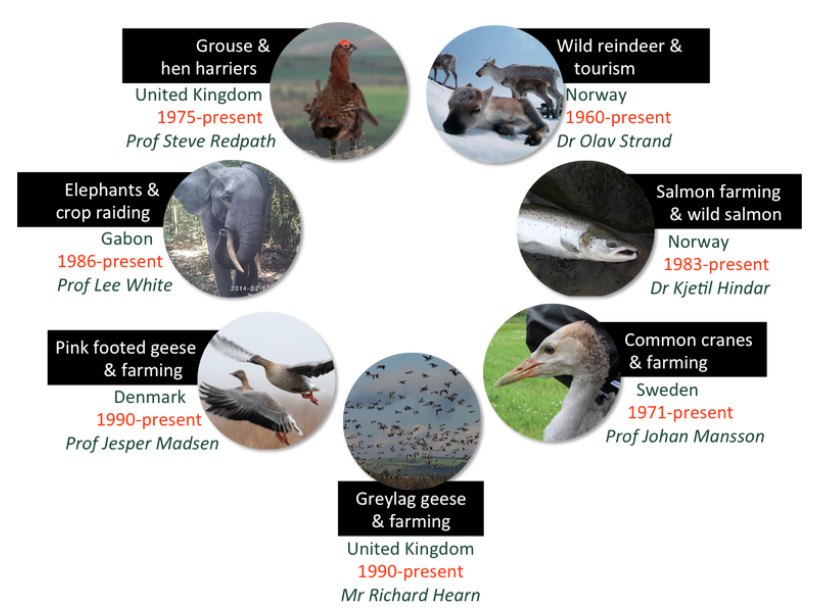
\includegraphics[scale=0.5]{confoobio-cases.png}
	\caption{The cases of conservation conflicts on which the ConFooBio project is focused.}
	\label{confoobio}
\end{figure}
%, or Rhinos conservation and illegal poaching for Ivory in south Africa \citep{glynatsi2018evolutionary}.
%Resolving these conflicts requires effective management strategies.
%Management strategy: a sequence of actions on the system in order to achieve goals.\\
%Yet, ecosystems dynamics are highly complex and interconnected, their evolution very difficult to anticipate.
%\subsection{Divergent interests between stakeholders}
In these conflicts, the divergence of stakeholders preoccupations makes conservation more challenging, as people impacted by a protected population's growth are more likely to defect protection policies.
That is why considering every stakeholder interests is essential for a management policy to be sustainable \citep{redpath2013understanding}.\\
% BD: I'm not sure if meeting every stakeholder interest is essential, so much as considering every stakeholder interest?x
%Indeed, farmers are usually more interested in the yield they live on, then in the survival of the species that is part of its decreasing.
%
%\subsection{MSE}

Management Strategy Evaluation (MSE) is a framework that describes the process of Adaptive Management in situations of conservation conflict.
It decomposes the problem into four main parts: manager's policy updating, user's harvest strategy, the species population and the mode of estimation of the population (see figure \ref{msediagram}).
\begin{figure}
	\centering
	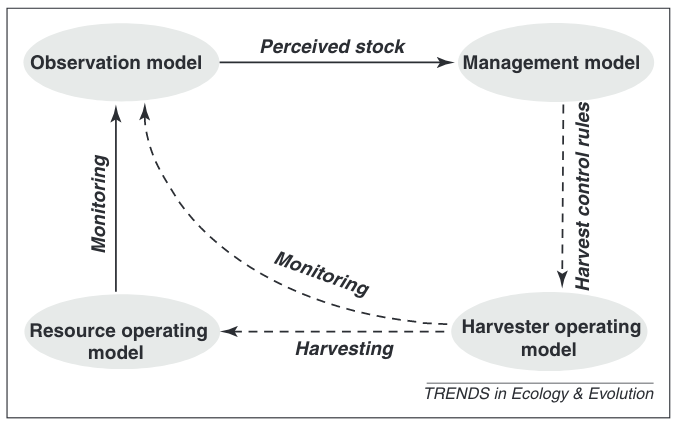
\includegraphics[scale=0.5]{msediagram.png}
	\caption{Flow diagram for the management strategy evaluation framework. This comprises a resource operating model (simulating the 'true' population biology of the species), the observation model to monitor the species (with error) and the management model, using the perceived stock to create and implement the harvest control rules. \citep{BUNNEFELD2011441}}
	\label{msediagram}
\end{figure}
This structure isolates uncertainty at four main levels: decision-making under uncertainty for managers and users, the population's response,

% BD: I think that it would be helpful to make the four main parts in the previous sentence link more explicitly to the four different types of uncertainty in this sentence. The information is there, but it might be difficult for an unfamiliar reader to figure out which type of uncertainty goes with which sub-model. Note that each type of uncertainty also has a unique term, as in \cite{BUNNEFELD2011}

%links between components of the ecosystems,
and its estimation.
%politics
%All the problems it deals with.
Also, the circular structure is adapted to the heuristic updating of management policy.

With such divergent interests, reaching a consensus on a target size for the population can be an unproductive process, and prevent the situation from changing in a more equitable way \citep{peterson2005conservation}. 

% BD: Maybe 'challenging' rather than 'unproductive'? Reaching consensus would definitely be productive, but such consensus is difficult to achieve in practice. How the second part of this sentence follows from the first ('and prevent the situation [...]') also isn't entirely clear. Might want to start a new sentence here and guide the reader through the logic of how the process can impede a transition to a more equitable situation ('equitable' presumably for the stakeholders involved)

Unlike consensus-based approaches, placing managers and users into two different parts recognizes different interests and expectations for conservation, and describes a goal-oriented behaviour. % BD: I think the logical link between separating manager and user sub-models and goal-oriented behaviour needs to be made stronger here, or perhaps these are separate points?
It was successfully implemented in fisheries, and then applied to terrestrial animals conservation \citep{BUNNEFELD2011441, bunnefeld2013incentivizing}.
% BD: Need to clarify what 'it' is referring to here (MSE, the separation of manager and user submodels?). Maybe a bit more detail into the background of MSE in fisheries (when, why it was developed) and then terrestrial systems could be helpful -- also, this texts seems more to do with adaptive management than conflict. I think it would help to separate them more clearly, in that you can have adaptive management in the absence of conservation conflict, and also conservation conflict without adaptive management. But the two subsections 'Adaptive management' and 'Conflicts' don't seem to be clearly separated.
%Still need to establish targets.

\subsection{Modelling}

Since an accurate prediction of these socio-ecosystems' response is hardly possible, any conservation frameworks benefits from a modelling approach. % BD: I see how the logic flows from the previous section, but I think it would be better to connect this more explicitly to the uncertainty. E.g., "Given the uncertainty inherent to all aspects of ecosystem management under conservation conflict, accurate prediction of system dynamics is especially difficult. Hence, a modelling approach to predicting system dynamics requires an explicit consideration of uncertainty" Something like this to make it clear to readers why perfect prediction in these systems is impossible.
Indeed, conceptual models allow for the rapid exploration of different scenarios under certain hypotheses, thus being very useful decision-helping tools. % BD: I'm not entirely sure what you mean here by 'rapid exploration of different scenarios'; does this refer to simulation of system dynamics (population density changes, human decision-making consequences) under different starting conditions or assumptions? What kind of hypotheses? I don't think unfamiliar readers will be able to follow this easily.
%
%\subsection{Different models used in literature}

%Ref: schluter2012, rumpff2011 (dealt with uncertainty by implementing different scenarios), bainbridge2017.
For example, \cite{rumpff2011state} used a Bayesian network to model the transitions between the possible state of a landscape according to a policy, to plan for the restoration of different protected areas previously damaged by human activity. % BD: Clarify what is meant by 'state of a landscape'? E.g., land use, biodiversity, forest cover?
The book from \cite{schluter2012new} threw the stones of socio-ecological modelling in order to manage conservation involving human compliance (an extensive list of studies using modelling in conservation is presented in chapter 2.1).
But, the high diversity of models highlights the lack of common framework, to which MSE is a strong candidate. % BD: I think this case needs to be made more strongly. First, is it possible to still have a high diversity of models *and* a common framework (i.e., unclear what kind of diversity of models is being described). Also, why is a common framework preferable to set of diverse, tactical, models that address an isolated case study? Assuming a common framework is important for addressing issues in volving conservation conflict, what is the advantage of MSE over other candidates?
In the conclusion, the authors also stated that a proper modelling framework for conservation conflicts needs human decision-making modelling, because unforeseen defection is one of the main causes for failures.\\
%
%\section{Decision-making modelling}

Game Theory (GT), introduced by John Von Neumann and Oskar Morgenstern in 1944 in the book "The Theory of Games and Economic Behavior", is the leading framework for decision-making modelling.
%\subsection{Game theory}
\cite{myerson1997game} describes GT as follows: "\textit{the study of mathematical models of conflict and cooperation between intelligent rational decision makers [which choices] affect one another welfare}". % BD: 'in which choices'? 
\textit{Games} are simplified vision of actual conflicts, because the actual complexity is unreachable, and can prevent from understanding the fundamental issues of conflict. %and cooperation. % BD: Isn't this true for all modelling though? Models are simplifications of reality, always wrong but often useful?
As any other scientific work, game models deliberately omit less relevant details of actual situation to allow the study of particular phenomenon in the scope of a particular question.

In these games, players act in order to maximise the expected value of the game's outcome, the so-called \textit{utility}.
Utility is not necessarily quantified as a monetary pay-off, it can be seen in many different ways, e.g. time, effort saved, well-being, happiness, \textit{etc}, and even a mix of them).

A game theoretical perspective can provide insights about: "the strategies different stakeholders will likely adopt given their objectives, [\dots] the range of possible outcomes, [\dots] and whether an optimal or satisfactory solution for all stakeholders can be reached simultaneously" \citep{COLYVAN20111246}.
It was first used in Biology in \cite{maynard1973logic} to investigate the evolution of animal strategies in con-specific fights.
%Definition of the key concepts like utility. Ref: myerson1997.
%\subsection{Application to conservation conflicts}
\cite{COLYVAN20111246} investigated theoretical applications of the four main types of games (simple, chicken, stag and prisoner games) to Adaptive Management, but its actual implementation for conservation purposes is fairly novel. % BD: I'm not sure what you mean by 'theoretical applications'. 
\cite{glynatsi2018evolutionary} modelled the conflict over rhinos protection and illegal poaching for ivory as a common-pool resource problem, to assess which proportion of rhinos should be de-horned to minimize their killing, according to poachers being unconditional or selective killers. %(figure \ref{rhino-poachers-game}). % BD: This sentence seems seems out of place; it's a good example of an application of game theory to conservaation conflict, but it's not really a conclusion of the paragraph. It might be useful to go through a bit more of the literature for the limited cases in which game theory has been applied to conservation, with some sort of summary or concluding thought on what has or has not been learned from this scant literature. 
%\begin{figure}
%	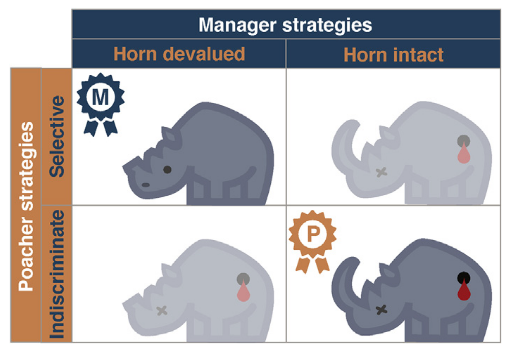
\includegraphics[scale=0.5]{rhinos-poachers-game.png}
%	\caption{The game between rhino manager and rhino poachers. The system settles to one of two equilibriums, either devaluing is eff ective or not. N.E. Glynatsi et al.}
%\end{figure}

And finally, a model developed on MSE framework, including decision-making modelling within Game Theory, was introduced in \cite{duthie2018}.

\section{GMSE}%Ref: duthie2018gmse. emphasize on its novelty.

\subsection{Formalisation of MSE framework}

%describe how it falls in MSE framework, how it deals with uncertainty at each level, consensus biases, long term foreseeing.
%At four main levels: population dynamics, links between components of the ecosystems, type of estimation of the population, making the right decision without knowing precisely the outcomes, reaction of the users, politics, response of the system, ...\\
%Explain clearly what it is meant for.
GMSE is a formalisation of MSE framework, assigning each part a mathematical model. % BD: I wouldn't necessarily say that GMSE is a formalisation of the framework so much as a generalisation of the traditional framework that integrates game theory and AI. The default models of the GMSE software include some mathematics, but are otherwise individual-based.
It aims at exploring the long-term consequence of a given management strategy, in order to test its effectiveness, and highlight problems managers would eventually not have thought of.
GMSE can be applied both for research \citep{cusack2018time}, and application to conservation conflict cases \citep{bainbridge2017goose}.
% BD: It might be useful to break this up into sub-sections, or walk the reader through each sub-model in paragraph form. Good focusing on the default population model as individual-based and spatially explicit, but you might need a bit more detail to explain this to readers who are unfamiliar with IBMs -- what's the difference between an IBM and a mathematical model, and what are its advantages and disadvantages?
Concerning the mathematical models, the population changes at each time step according to a spatially explicit, individual-based, population dynamic model.
Each individual is born, moves, and dies according to probabilities drawn in defined laws to account for the uncertainty linked with population dynamics.\\
The population is monitored according to different definable techniques, some of which includes probabilities of detection, thus accounting for the uncertainty about the accuracy of monitoring.\\ % BD: You might want to tie this in with the 'virtual ecologist' approach in the literature. See: 
% (1) Zurell, D., Berger, U., Cabral, J. S., Jeltsch, F., Meynard, C. N., Münkemüller, T., ... Grimm, V. (2010). The virtual ecologist approach: Simulating data and observers. Oikos, 119(4), 622–635. https://doi.org/10.1111/j.1600-0706.2009.18284.x 
% (2) Nuno, A., Bunnefeld, N., & Milner-Gulland, E. J. (2013). Matching observations and reality: Using simulation models to improve monitoring under uncertainty in the Serengeti. Journal of Applied Ecology, 50(2), 488–498. https://doi.org/10.1111/1365-2664.12051 
% (3) Grimm, V., Wyszomirski, T., Aikman, D., & Uchman'ski, J. (1999). Individual-based modelling and ecological theory: synthesis of a workshop. Ecological Modelling, 115, 275–282.
The manager model can be parametrized to reflect its conservation goals. % BD: Maybe a bit more on what these conservation goals are (linking to your earlier point about targets).
It uses the information from the monitoring to set a policy.
A policy is a set of possible actions associated with a cost for their performing. % BD: Technicality, but I would not say that a policy is a set of possible actions, but rather a set of actions drawn from a list of all possible actions available (in GMSE). 
The manager has a given budget, and implementing a policy implies a cost for them.\\ % BD: Might be easier to start with the manager's budget, then work to the specifics of policy actions, including the specific actions available.
The user model is individual-based, and each user can be parametrized to reflect its interests concerning the population.
There can be any natural number of users, and users' decision-making and actions are modelled independently.
Each has a given budget and acts according to the number of actions they can perform according to their cost set by the manager, in order to achieve his/her goal (figure \ref{gmse-diagram}). % BD: Should link this back to policy, and make clearer that users incur a cost for each action which varies according to how the manager has set policy.
\begin{figure}
	\centering
	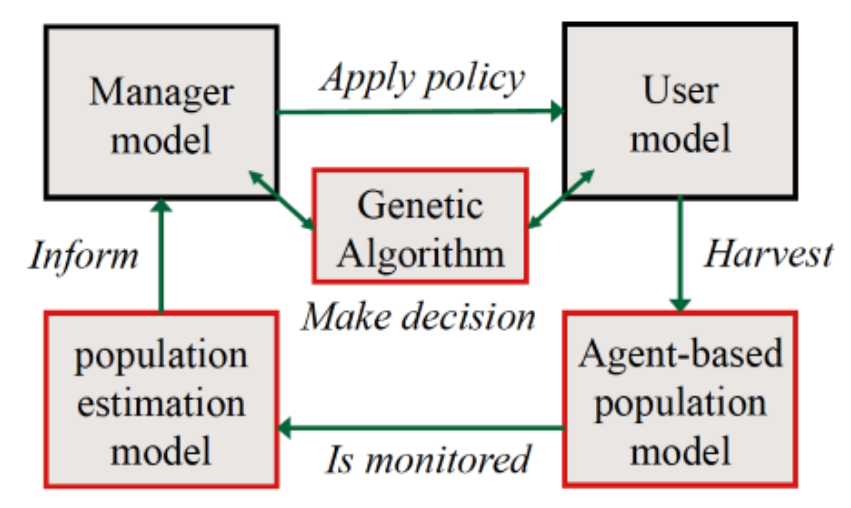
\includegraphics[scale=0.35]{gmse-diagram.png}
	\caption{Flow chart of GMSE current version. Red outlines indicate stochastic models.}
	\label{gmse-diagram}
\end{figure}
%\subsection{First IBM in conservation}
%
%"Individualbased
%models (IBMs; also known as agent-based models) are
%used to model the behaviour of a system at an individual level
%by specifying simple rules for agents and allowing them to
%interact. These models allow for complex behaviour to emerge
%from simple interactions, though this comes at some cost to
%interpretation and analysis." Ref: hamblin2012parctical.

According to MSE framework, a policy is effective when, after the chosen period of management: % BD: Citation? I think these are good criteria, but are they really part of the framework, or did  you develop them yourself?
\begin{itemize}
    \item The population (i) does not go extinct and (ii) stabilizes around the conservation target.
    \item The users' yield reaches a satisfactory percentage.
    \item All users have comparable yield percentages.
    \item The spatial distribution of the resource is equitable between users' lands.
\end{itemize}
If these condition are fulfilled, there should not be any reason left for conflict to persist.

\subsection{Decision-making artificial intelligence}

%Genetic algorithm. Very accessible worded explanation. ref: hamblin2012practical\\
%How is it suited to human decision-making?\\
%Also used in solving game theoretical problems. Ref: Maynard Smith 1982.\\\
%An example of interaction between IBM and genetic algorithm was in hamblin2009, where the parameter governing the interaction rules in foraging ants where allowed to evolve through a GA.
The manager's and the users' decisions are made by calling a Genetic Algorithm (GA) - a form of Artificial Intelligence (AI).
Initially, GAs were used to model the evolution of allele frequencies in a population under stochastic recombination and mutation. % BD: Citation?
It has previously been used in combination with an individual-based model in a ant collective foraging model, where the parameter governing the interaction rules was allowed to evolve according to a GA \citep{hamblin2013practical}. % BD: I can't find the ant collective foraging model in hamblin2013practical -- is there another citation to this?
Although this algorithm was not exactly successful in mimicking evolution, it inspired a new kind of Artificial Intelligence.

Here, a population of random strategies of a given size is initiated, and then allowed to change through stochastic mutation and crossing-over. 
Each strategy's fitness to the decision-maker criteria is assessed, and the fittest are allowed to reproduce.
The process is repeated until the increase in fitness between the current fittest stategy and the previous one falls under a defined threshold and some minimum number of GA generations have passed.

The GA is particularly well fitted to human decision-making in this context, because due to the complexity of the problem, the decision-maker does not know in advance the best choice, but can judge if a choice is better than another.
Furthermore, humans are usually not able to explore all the possibilities to choose the best one, they rather select the best among the one they could think of.
%
%\subsection{Opportunities for further development}
%%
%%\subsubsection{Theoretical}
%
%%Agents act independently, which is very unlikely. REF???!!\\
%GMSE is very new and have many opportunties to further development.
%For example, in the current version, the users act independently, regardless of their neighbours' behaviour.
%This is very unlikely, as seen in the role-play games performed in \cite{redpath2018games}.
%Also, Game Theory explicitly showed how crucial was the ability to know the other players' strategy to get the most out of the game's outcome.
%%%Different types of conservation interests.
%Besides, at the moment, the manager's only goal is to maintain the population, but \cite{holmes2017understanding} showed that the interests of conservationists can be broader and more complex.
%%%Would be interesting to implement.\\
%%%Does not consider the do nothing option which is sometimes interesting.\\
%Another feature that could be explored is the frequency of policy updating, currently quite rigid, as the manager acts whenever she/he is meant to, regardless of the situation.
%%\subsubsection{Computational}
%%On the computational side, computing time increases greatly with the number of stakeholders, due to the individual-based approach.
%%%Lacks machine learning to be a proper artificial intelligence.
%%Furthermore, it is now complicated to speak about AI without including Machine Learning, yet Genetic Algorithm is not a structure that can be trained.

\section{Research Questions}
%They have to be very closely related to conservation (to avoid making it a mere modelling project)
I will focus on an actual case study of conservation conflict to keep GMSE development into a down-to-earth situation, and parametrize simulations with actual measures from the field.
I chose the case of conflict over geese population and farming on the Isle of Islay (Scotland) as it is a well documented case, with very accessible data within the team.

\subsection{Case study: Geese}

%Description. Ref: mason2017, brainbridge2017.
The endangered status of geese was recognised during the 1940s, and is believed to result from a combination of hunting for food and recreation, systematic persecution and the disruption of the Second World War. % BD: I'm told that hunters prefer the term 'recreation' to 'sport', though I'll confess that I'm entirely sure I understand what the difference is.
In the 1980s, all geese species population numbers increased significantly, most likely as a consequence of improved protection, paired with land-use and climate change \citep{mason2017changing}.
But this rise in population started a conflict with farmers in Special Protection Areas, as geese were intensely grazing their crops.
%Especially for farmers owning culture in Special Protection Areas required by the European Bird Collective.
The first arrangements between the state and these farmers concerning geese control were made in the early 1990s, in the form of payments from government for farmers to allow undisturbed grazing on certain areas, and scare them away in others areas.
Yet, some populations continued to increase, and farmers started to consider the compensation too low for the damages caused.
But Scottish government refused to increase them for financial reasons \citep{bainbridge2017goose}.
%Farmers then started to control the population by means unapproved by the conservation scheme .

%Its attributes (liked with the limits of GMSE).
This case is particularly adapted to work on the development of GMSE, because it is a small-scale case of conservation conflict, involving a tractable number of neighbouring users who are very likely to interact in different and interesting ways.
It is already a case of interest for Scottish National Heritage (SNH), and part of the ConFooBio project, so the goose population, along with the updates in the conservation policy, have been regularly monitored for years.
Furthermore, this situation could clearly benefit from the results of this project, and would be an interesting way to test once again the applicability of GMSE to actual cases.
%from now on always speak about goose, state and farmers to settle the problem in the context of geese

\subsection{How does flexibility in policy updating frequency affect geese management strategy efficiency?}
%\subsubsection{Action threshold}
%%Currently in GMSE, a parameter sets the number of the manager's interventions per time step. Rigid, insensible to the situation, action if pop $>$ ou $<$ target, regardless of the size of this difference. acting even if the population if only a few individuals from the target.\\
%First, fixed deviation from manager's target as an action threshold. has to be relative the the population size though, if population size is 100, 50 individuals missing or extra is very concerning, yet it is less if population size is tens of thousands. For example I could test thresholds of 1, 5, 10, \dots \% of target.\\ 
%Quantitative assessment of the impact on the "quality" of the policy over repeated simulations for increasing threshold values: mean deviation from manager's target? Impact? Conflict reduction? number of extinctions? (Is there a chance that the result will be the same as the manager intervention frequency?)\\
%Dynamic threshold? A function of deviation from target, or conflict intensity, that would modify the action threshold.\\
%Waiting could imply saving a certain amount of budget for next step. Something that could also concern the users, maybe highlighting a best time to act.
%Recently introduced in iacona2017evolutionary: optimal delay before using funds.
Optimal growth in finances, or plant, sometimes includes doing nothing. % BD: I think this could be clearer -- do you mean that the best action to take to manage a population (or a business, perhaps) is to not attempt a change in action (i.e., "if it's not broken, don't try to fix it").
More precisely, to invest less resources than usual in buying (balancing consumption and capital investment) or reproduction (less investment in seeds or flowers and more in root stock or growth, waiting for a less unsuitable or competitive time) for a certain amount of time. % BD: I like how you've explained this -- I wonder if it might be useful to find some examples in history (conservation or others) in which not doing anything would be preferable to any other action? There are of course, plenty of examples in which doing nothing would have been preferable to what was *actually* done (cane toads in Australia come to mind -- which were originally meant to control the cane beetle, but were wildly ineffective), but I can't think of anything off hand in which leaving things alone was concluded to be the best option -- they must be out there in the literature somewhere.
Since the problems conservation is dealing with are often irreversible, managers are used to invest financial resources in acting as soon as they get them.
%Optimal growth concept applied to management strategy shows that investing in other domains than policy application is sometimes more profitable for conservation goals, if the possible outcome outweigh the increase in threat in the meantime.
%By doing nothing, authors mean invest in other domains than policy application, such as research, monitoring, or even other lucrative placements.
%But only if the possible outcome outweigh the increase in threat in the meantime.\\
Indeed, the complexity of conservation problems results in temporal heterogeneity, so acting can be more efficient at certain moments than others, if the possible outcome outweigh the increase in threat to the protected species in the meantime.
%Just as conservation outcomes can be improved by "identifying the most efficient locations to act in space",
Thus, finding the best time to act could lead to more efficient management strategies \citep{Iacona2017waiting}.
%
%%\subsubsection{Calculus of impact}
%In \cite{gordon2011assessing}, the efficiency of offsetting is assessed by the "impact" of the policy implementation.
%It is the difference in the amount of native habitat loss when offsetting or not.
%This could be a interesting condition to assess whether manager should update the policy at this time or not. PAS A LA BONNE PLACE

Currently in GMSE, a parameter sets the number of the manager's interventions per time step, and according to \cite{duthie2018}, the number of extinctions over several simulations decreases exponentially with increasing frequency of manager intervention.
%So, I suspect it is going to show that doing nothing is not sustainable as a policy in itself. Surprise!
But does this mean acting as soon as possible is always an efficient strategy?\\ % BD: This is good, and it might be useful to also think about what constitutes 'efficient strategy' in this case -- this will almost certainly relate to both the strategy objectives (e.g., how close to the target density do you want to be, or how much do you want to minimise the extinction risk) and the use of time and money (budget, perhaps in this case). You could make the argument that although a strategy might maintain the population most closely to the target density when a lot of effort is expended (in terms of time and money spent), the gains in terms of minimising the deviation from target become more expensive than they are worth in some cases, and it would therefore be more efficient to decrease effort and allow the deviation from target to increase so that energy could be spent elsewhere. Addition, if budget can be saved, it might actually minimise the deviation from target even further by allowing a manager to draw from a larger budget when doing so is really necessary.
%I will answer this question by implementing new features in GMSE, and assess the efficiency of management strategies using them.

To answer this, I will implement a `doing nothing' option in GMSE, as a bypass of policy updating under certain conditions at a given time step. % BD: I would make clear that this development is actually a new policy option, effectively, for the manager -- you're not just telling the simulatoin to do nothing, but allowing the manager to not set policy and instead save resources for future decision-making outcomes.
The most intuitive condition would be the deviation of estimated population from the manager's target.
For now, the manager updates the policy whenever they are meant to, even if the estimated population is only a few individuals away from the target.
To loosen this condition, I will implement an action threshold $A$ based on $D$, the ratio of estimated population size to manager's target size.
If at this time step, $|1 - D| < A$, the policy will not be updated, meaning that the manager would act only if the population exceeds or goes under its target by a certain value set by $A$. % BD: Nice idea! 

First, $A$ will have a fixed value along the conservation scheme period.
To quantitatively assess the effect of this strategy on management efficiency, I will select a set of relevant values for $A$, and run multiple simulations for each of them - probably a hundred replicates per $A$ values.
For each $A$ value, I will gather different informations from the simulations, according to the MSE criteria for an efficient management strategy:
\begin{itemize}
	\item The number of simulations in which the goose population went extinct, divided by the number of replicates, to estimate a probability of extinction.
	\item The mean deviation of the actual goose population from conservation target over the conservation scheme period, averaged over all the replicates.
	\item The mean total crop yield percentage across the conservation scheme period, averaged over all the replicates.
	\item The mean variability in crop yield percentage across the different users, averaged over all the replicates.
	\item The mean variability in the number of geese per land unit across the different users, averaged over all the replicates.
\end{itemize}
I will use these measures to compare the effectiveness of the management strategy according to the value of $A$, and eventually highlight the most efficient one.\\ % BD: This all looks good, but I would be surprised if any value of $A < 0$ would result in better management in the absence of some sort of trade-off. Even given the extreme scenario in which the manager's policy is already ideal and $D = 1$, the GA should then be able to find the same strategy that got to this situation of good management. If there's no cost to finding it again, then it's difficult to see how the option to look would decrease any of the above bullet points. My intuition would be that optimal $A$ would be most usefully defined in terms of the cost of changing policy.

I have also thought of another way to find an optimal value for $A$, involving a more dynamic way to set it during the conservation scheme period.
The value of $A$ could be a Gaussian, or a two-tailed stair function, of a variable describing the situation ($|1-D|$ for example), centred on a maximum value for $A$.
That way, if the situation is concerning at this time step, it could mean that the previous $A$ value was too high, thus the manager can adjust it to react more sensibly from now on.

I will run multiple replicates for different parameters values for the link-function between $A$ and the variable describing the situation.
From the simulation output, I will assess the evolution of the mean $A$ value over the replicates at each time step, along the conservation scheme period.
This will eventually show the emergence of an optimal value for the action threshold according to the link-function's shape and parameters.\\

Finally, an interesting feature to add to this exploration would be the ability for the manager to save some budget for next time step if she/he decided not to act this time step.
I could assess the efficiency of the policy according to different percentages of budget saving, with the same method as previously. % BD: It could also be interesting to consider a trade-off between investment in policy implementation (under the conditions that you describe above) and investment in observation. Maybe in time steps where the cost is not used for implementing policy (because the population is close to target), more resources could be devoted to getting a more accurate estimate of the true population size (better observation model -- e.g., observe more space or mark-recapture more individuals).
%According to \cite{duthie2018}, the number of extinctions over several simulations decreases exponentially with increasing frequency of manager intervention. %So, I suspect it is going to show that doing nothing is not sustainable as a policy in itself. Surprise!
%But does it means acting as soon as possible is is a sustainable strategy?

%
%\subsection{Including human values in adaptive management}
%
%All conservationists have different goals according to their values, it would be interesting to implement this. Using the framework from futureconservation.org, I could use quantitative measures of conservationists values and attribute utilities accordingly, and assess if it indeed produce the expected results. Users yields and population size according to the value on nature - people axis, and to conservation - capitalism one. 

\subsection{How to manage geese population efficiently taking into account interactions between stakeholders?}

The main research goal of this project is to allow the decision-making AI to consider interactions between agents.
In GMSE current version, the users act independently, regardless of their neighbours' behaviour.
This is very unlikely, as seen in the role-play games performed in \cite{redpath2018games}.
Also, Game Theory explicitly showed how crucial was the ability to know the other players' strategy to get the most out of the game's outcome \citep{hilbe2018evolution}.
I will take advantage of answering the first research question to get familiar with the case study, as well as GMSE code, in order to find out what kind of interactions are at play here, and how to implement them within the existing structure of the software.
After that, I will be able to assess how it affects the way managers make policies.
%This is a real challenge because, to my knowledge, it has not been explored before.

\subsection{Next challenges}

GMSE being a completely novel software, there are still many ways to keep on developing it.

%\subsubsection{Computational}
From a computational point of view, computing time increases greatly with the number of stakeholders, due to the individual-based approach crossed with the systematic calling of the Genetic Algorithm.
This could be improve using parallel computing.
With the adapted software and code language, this technique allows to make many similar tasks simultaneously instead of in sequentially, thus highly increasing the throughput (number of operations per time unit).

Furthermore, it is now complicated to speak about AI without including Machine Learning, yet Genetic Algorithm is not a structure that can be trained.
To turn the decision-making AI into a learning structure, the team thought about a Neural Network (NN) in the shape of a map.
Given a variety of inputs, the NN would be able to output a land-use decision map.
The NN would be trained with data from numerous behavioural games performed within the ConFooBio project.
Once coded, this new version of GMSE could be compared to the previous one in terms of ability to manage conservation conflicts.
%\section{Expected outputs}
%
%At least a paper on the action threshold, a talk in Newcastle, a poster in winter symposium, a participation at the Trondheim workshop. Updated version of GMSE. Field work for SNH, possibly in the policy team to which Aileen is close.

\newpage
\bibliography{10WRbib}
\nocite{*}

\end{document}
